\documentclass[a4paper,10pt,twocolumn]{article}

\usepackage{amsmath}
\newcommand{\td}{\mathrm{d}}
\newcommand{\te}{\mathrm{e}}
\newcommand{\ti}{\mathrm{i}}
\newcommand{\sinc}{\mathrm{sinc}}
\usepackage{tikz}

\begin{document}

\section{Analytical singular integrals of the Poisson kernel}

\subsection{2D case}

\begin{equation}
G(r) = -\frac{\ln |r|}{2\pi}
\end{equation}

\subsubsection{Collocation over constant line}

\begin{equation}
\int_{-d_1}^{d_2} G(r) \td r
=
\frac{d_1 + d_2 - d_1 \ln |d_1| - d_2 \ln |d_2|}{2\pi}
\end{equation}

\begin{multline}
\frac{\partial}{\partial n_x}
\int_{-d_1}^{d_2} 
\frac{\partial}{\partial n_y}
\frac{-\ln |r|}{2\pi}
\td y \\
=
\frac{\partial}{\partial z}
\int_{-d_1}^{d_2} 
\frac{-1}{2\pi r} \frac{(y, -z) \cdot (0,1)}{r}
\td y \\
=
\frac{1}{2\pi} \frac{\partial}{\partial z}
\int_{-d_1}^{d_2} 
\frac{z}{\left(y^2+z^2\right)}
\td y \\
=
\frac{1}{2\pi} \frac{\partial}{\partial z}
\left[
\tan^{-1}\left(d_2/z\right)
-
\tan^{-1}\left(-d_1/z\right)
\right]
\\
=
\frac{1}{2\pi} \frac{\partial}{\partial z}
\left[
\tan^{-1}\left(d_2/z\right) + \tan^{-1}\left(d_1/z\right)
\right]
\\
=
\frac{1}{2\pi} 
\left[
\frac{-d_2}{d_2^2+z^2} + \frac{-d_1}{d_1^2+z^2}
\right]
\\
\to
\frac{-1}{2\pi} 
\left[
\frac{1}{d_2} + \frac{1}{d_1}
\right]
\end{multline}


\subsubsection{Galerkin over constant line}

\begin{equation}
\int_{0}^{d} \int_{0}^{d} G(x-y) \td y \td x
=
d^2\frac{3-2\ln d}{4\pi}
\end{equation}


\subsection{3D case}

\begin{equation}
G(r) = \frac{1}{4\pi r}
\end{equation}

\subsubsection{Collocation over constant triangle}

\begin{equation}
\int_0^{2\pi} \int_0^{R(\theta)} \frac{r \td r \td \theta}{4\pi r}
=
\frac{1}{4\pi}\int_0^{2\pi} R(\theta) \td \theta
\end{equation}
%
The angular integral is split up into three integrals, each over one triangular domain.
One triangle is displayed below, $\bf x_0$ denotes the collocational point:

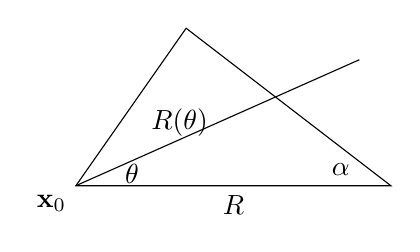
\begin{tikzpicture}[scale=2]
\path [draw] (0,0) node [anchor = north east] {${\bf x}_0$} -- node [anchor = north] {$R$} (2,0) -- (.7, 1) -- cycle;
\path [draw] (0,0) -- node [anchor = east] {$R(\theta)$} (1.8,.8);
\path (.25,-.05) node [anchor = south west] {$\theta$};
\path (1.8,0) node [anchor = south east] {$\alpha$};
\end{tikzpicture}

From the law of sines, $R(\theta)$ is expressed as
%
\begin{equation}
R(\theta) = \frac{R \sin(\alpha)}{\sin(\theta+\alpha)}
\end{equation}
%
using the identitiy
%
\begin{equation}
\int \sin^{-1}(x) \td x = \log \tan (x/2)
\end{equation}
%
the integral can be expressed (by summing for the three triangles) as follows:
%
\begin{equation}
I = \frac{1}{4\pi} \sum_{i = 1}^3
R_i \sin\alpha_i \left[ \log \left( \frac{\tan\left(\frac{\phi_i+\alpha_i}{2}\right)}{\tan\left(\frac{\alpha_i}{2}\right)}\right)\right]
\end{equation}


\begin{multline}
\frac{\partial}{\partial n_x}
\int
\frac{\partial}{\partial n_y}
G(r)
\td y
\\
=
\frac{\partial}{\partial z}
\int
\frac{-1}{4\pi \left(r^2_{2D} + z^2\right)}
\frac{({\bf r}_{2D},-z)\cdot({\bf 0},1)}{\sqrt{r^2_{2D} + z^2}}
\td {\bf y}
\\
=
\frac{1}{4\pi}
\frac{\partial}{\partial z}
\int
\frac{z}{\left(r^2_{2D} + z^2\right)^{3/2}}
\td {\bf y}
\\
=
\frac{1}{4\pi}
\frac{\partial}{\partial z}
\int_{0}^{2\pi}
\int_{0}^{R(\theta)}
\frac{r_{2D} z}{\left(r^2_{2D} + z^2\right)^{3/2}}
\td r_{2D}
\td \theta
\\
=
\frac{-1}{4\pi}
\frac{\partial}{\partial z}
\int_{0}^{2\pi}
\left(
\frac{z}{\sqrt{R(\theta)^2 + z^2}}
-
1
\right)
\td \theta
\\
=
\frac{-1}{4\pi}
\int_{0}^{2\pi}
\frac{\partial}{\partial z}
\frac{z}{\sqrt{R(\theta)^2 + z^2}}
\td \theta
\\
=
\frac{-1}{4\pi}
\int_{0}^{2\pi}
\left(
\frac{\sqrt{R(\theta)^2 + z^2} - \frac{z}{2\sqrt{R(\theta)^2 + z^2}}}{R(\theta)^2 + z^2}
\right)
\td \theta
\\
\to
\frac{-1}{4\pi}
\int_{0}^{2\pi}
\frac{1}{R(\theta)}
\td \theta
\end{multline}


\section{Analytical singular integrals of the Helmholtz kernel}

\subsection{3D case}

\begin{equation}
G(r) = \frac{\te^{-\ti k r}}{4\pi r}
\end{equation}

\subsubsection{Collocation over constant triangle}

The singular integral over a triangle is regularised by subtracting and adding the static ($k = 0$) part
%
\begin{equation}
G(r) = \frac{1}{4\pi r} -\ti k \te^{-\ti k r/2} \frac{\sinc(k r/2)}{4\pi}
\end{equation}
%
The static part is integrated analytically.
The dynamic part is regular and can be integrated using a low order Gaussian quadrature over the triangle.


\begin{multline}
G''_{n_x, n_y} = \frac{G}{r^2} \left[ 
\left(1+\ti k r\right)\left(n_x n_y + r'_{n_x} r'_{n_y}\right) \right. \\
\left. + \left(2 + 2 \ti k r - (kr)^2\right) r'_{n_x} r'_{n_y}
\right]
\end{multline}
%
and on a plane triangle
%
\begin{equation}
G''_{n_x, n_y} = \frac{G}{r^2} \left(1+\ti k r\right)
\end{equation}
%
We again subtract the static part, as well as the static Green's function $G_0(r)$ multiplied by $k^2/2$ to obtain a regular function represented by its Taylor series:
%
\begin{multline}
G''_{n_x, n_y} - {G_0}''_{n_x, n_y} - \frac{k^2}{2} G_0 = \\
-\frac{\ti k^3}{4\pi}
\left(
\frac{1}{3}
- \frac\gamma{8} 
+ \frac{\gamma^2}{30} 
- \frac{\gamma^3}{144} 
+ \frac{\gamma^4}{840} 
-\frac{\gamma^5}{5760} 
+\dots
\right)
\end{multline}
%
where $\gamma = \ti k r$




\subsubsection{Collocation over constant triangle}

The singular integral over a triangle is regularised by subtracting and adding the static ($k = 0$) part
%
\begin{equation}
G(r) = \frac{1}{4\pi r} -\ti k \te^{-\ti k r/2} \frac{\sinc(k r/2)}{4\pi}
\end{equation}
%
The static part is integrated analytically.
The dynamic part is regular and can be integrated using a low order Gaussian quadrature over the triangle.




\end{document}

